\chapter{Resultats}\label{chapter:resultats}
\vspace{-0.5cm}
En aquest capítol exposem els resultats del disseny i el desenvolupament del sistema sencer.

\section{Aplicació de servidor}
L'aplicació de servidor és la que més s'ha trigat en dissenyar i desenvolupar perquè el disseny de l'aplicació de client depen directament de la de servidor.

L'aplicació funciona com s'esperava.

A través de la interfície d'administració es poden fer fàcilment les gestions necessàries com són: afegir usuaris nous, afegir expenedors nous, gestionar els carrils dels expenedors ..., tot el que es requeria de poder gestionar en remot.

A la intefície d'administració només hi poden accedir els usuaris que tinguín permís d'administració, i això es pot gestionar des de la mateixa interfície.

\begin{figure}[H]
	\centering
	\begin{subfigure}[b]{0.45\textwidth}
		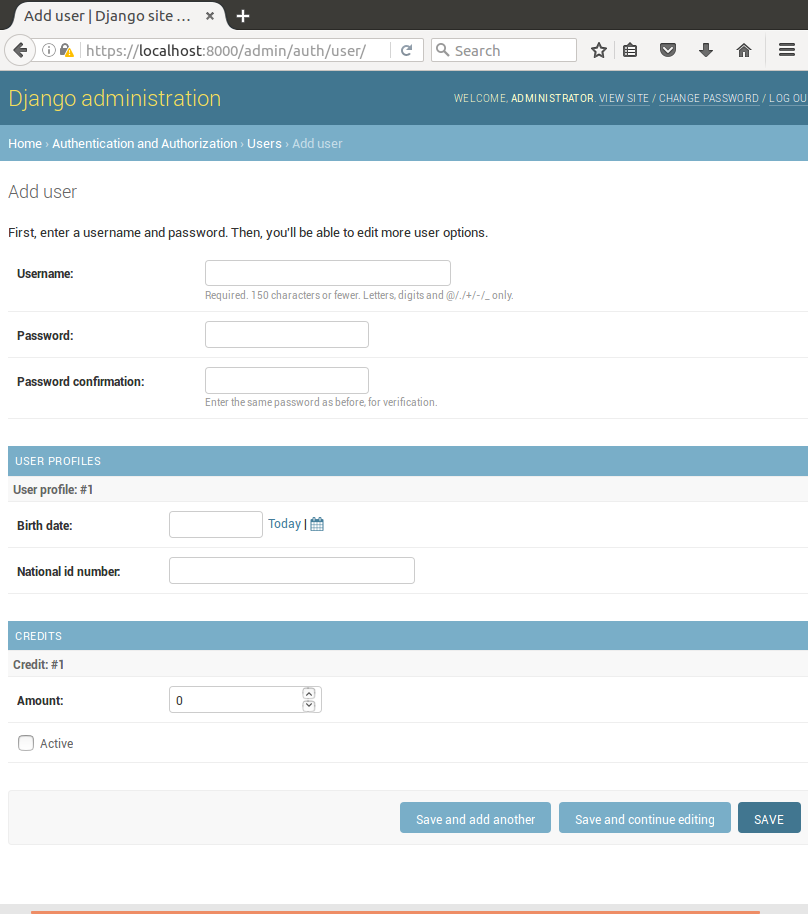
\includegraphics[width=\textwidth]{images/admin1}
		\caption{Interfície d'administració per crear usuaris}
		\label{fig:admin1}
	\end{subfigure}
	\hspace{0.5cm}
	\begin{subfigure}[b]{0.45\textwidth}
		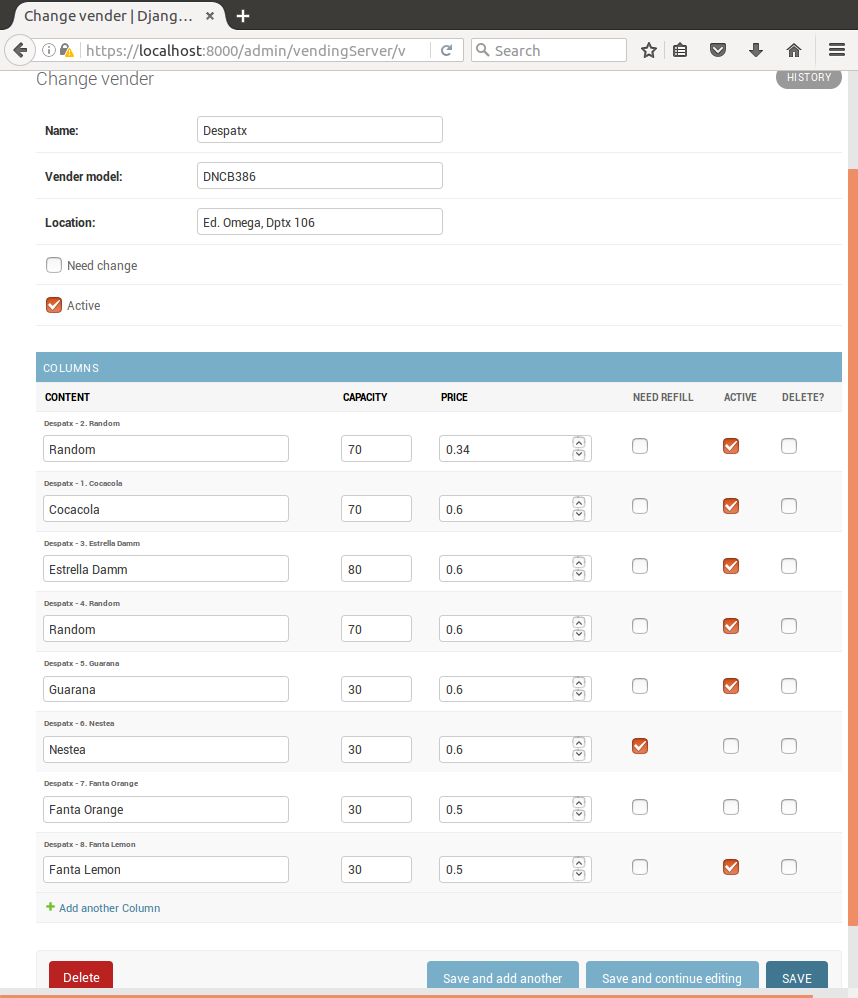
\includegraphics[width=\textwidth]{images/admin2}
		\caption{Interfície d'administració per gestionar els expenedors}
		\label{fig:admin2}
	\end{subfigure}
	\caption{Captures de la interfície d'administració de l'aplicació de servidor}
	\label{fig:intro-example}
\end{figure}

\section{Aplicació de client}
L'aplicació de client compleix els requeriments que s'han especificat.

No obstant, té un problema amb el lector de targetes: si l'aplicació es tanca de manera inesperada (per exemple, degut a un error d'execució inesperat), es perd la comunicació amb el lector, i no es pot recuperar fins que no se li fa un reset de l'alimentació al lector. Això és un problema de la llibreria que utilitzem per controlar-lo (nfcpy), ja que amb altres llibreries que s'han provat això no passava.

La interfície gràfica d'usuari no ha estat dissenyada per un dissenyador

\begin{figure}[H]
	\centering
	\begin{subfigure}[b]{0.45\textwidth}
		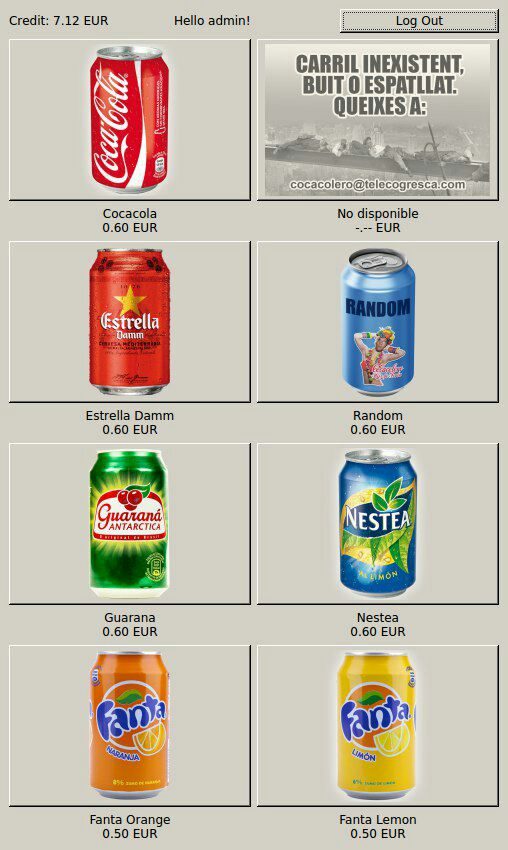
\includegraphics[width=\textwidth]{images/client_app1}
		\caption{Interfície d'administració per crear usuaris}
		\label{fig:admin1}
	\end{subfigure}
	\hspace{0.5cm}
	\begin{subfigure}[b]{0.45\textwidth}
		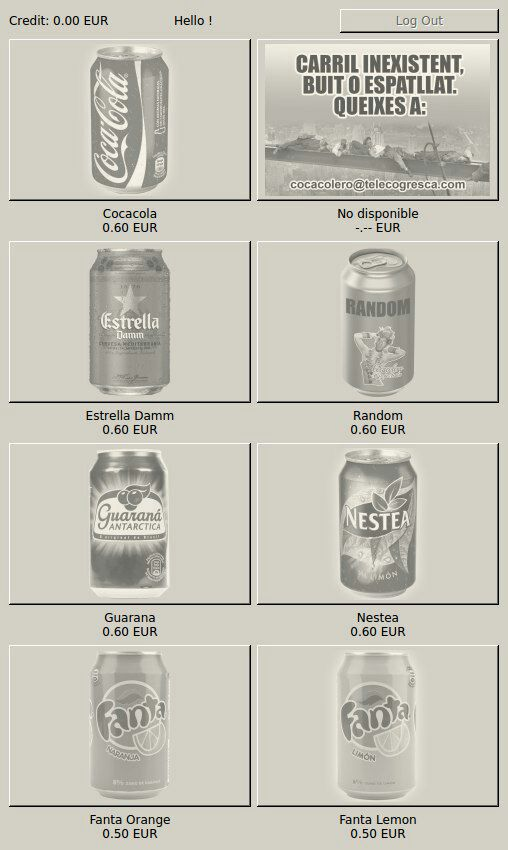
\includegraphics[width=\textwidth]{images/client_app2}
		\caption{Interfície d'administració per gestionar els expenedors}
		\label{fig:admin2}
	\end{subfigure}
	\caption{Captures de la interfície d'usuari de l'aplicació de client}
	\label{fig:intro-example}
\end{figure}

\section{Sistema de hardware}
El hardware en conjunt està desenvolupat. No obstant, per temes de calendari de l'associació (durant el mes de març l'expenedor està inaccessible, durant l'agost i part de setembre el despatx està tancat), no s'han pogut fer totes les proves que es volia fer.

Durant el quadrimestre s'han fet petites proves de concepte bàsiques amb èxit:
\begin{enumerate}
\item Provar d'expendre una llauna amb un relé activant-lo manualment.
\item Provar d'expendre una llauna amb els relés activats per l'aplicació de client.
\end{enumerate}

Més enllà d'això no s'ha pogut integrar el sistema dins de l'expenedor per problemes de calendari i falta de temps.

La unitat de prova ha estat desenvolupada amb èxit i és molt útil per transportar el sistema d'una manera còmode.

%\begin{figure}[H]
%	\centering
%	\begin{subfigure}[b]{0.45\textwidth}
%		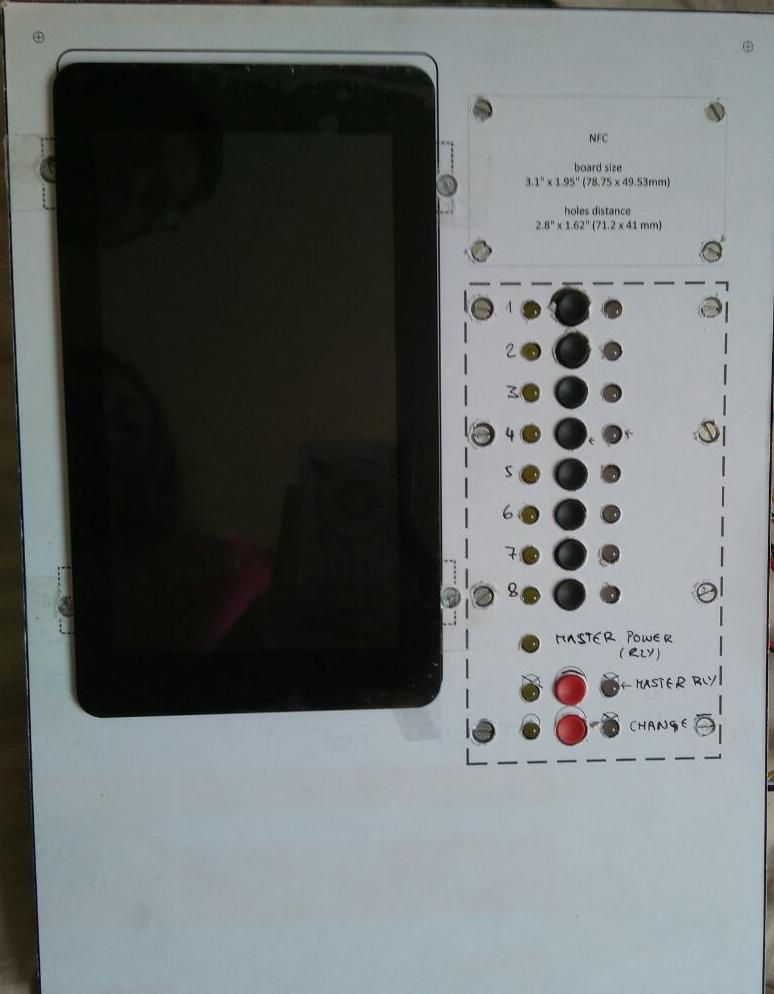
\includegraphics[width=\textwidth]{images/demonstrator_front}
%		\caption{Front de la tapa}
%		\label{fig:admin1}
%	\end{subfigure}
%	\hspace{0.5cm}
%	\begin{subfigure}[b]{0.45\textwidth}
%		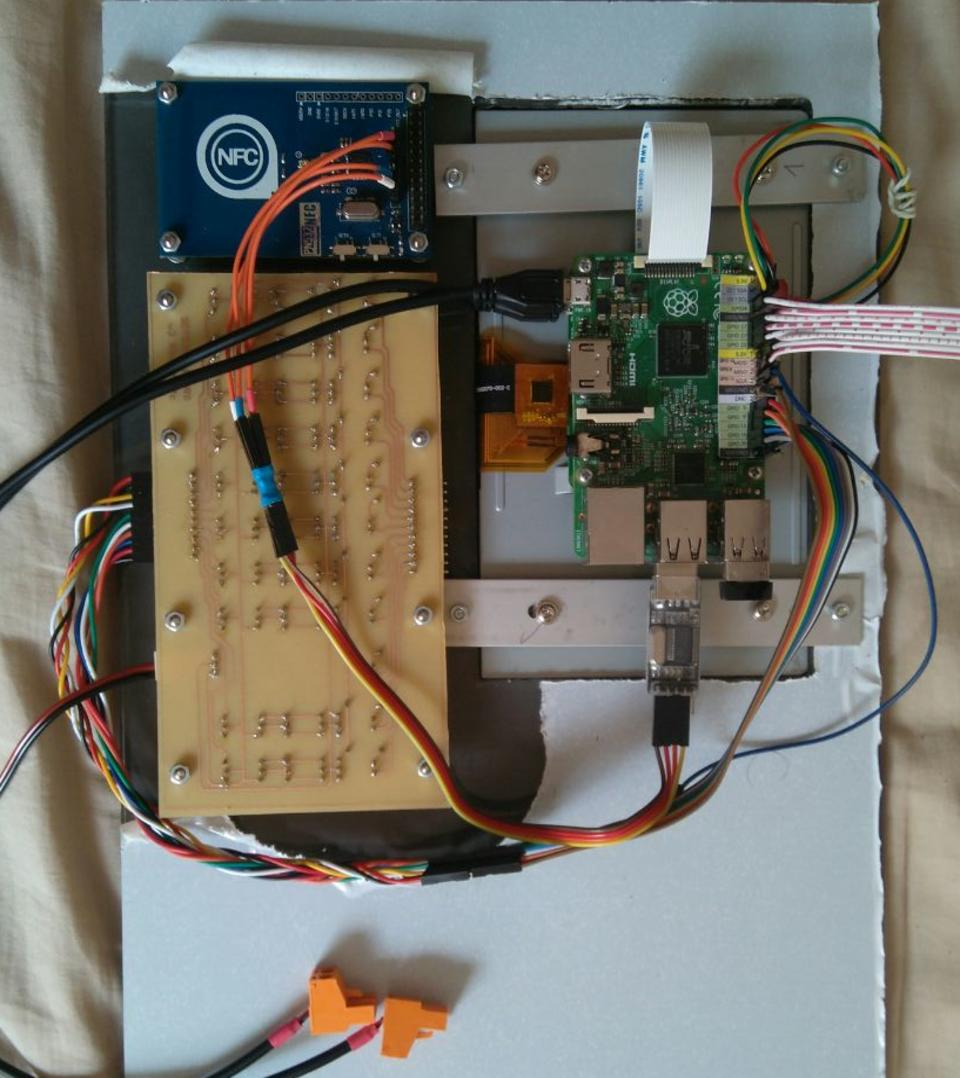
\includegraphics[width=\textwidth]{images/demonstrator_back}
%		\caption{Revers de la tapa}
%		\label{fig:admin2}
%	\end{subfigure}
%	\caption{Tapa de la unitat de test}
%	\label{fig:intro-example}
%\end{figure}

\begin{figure}
\center
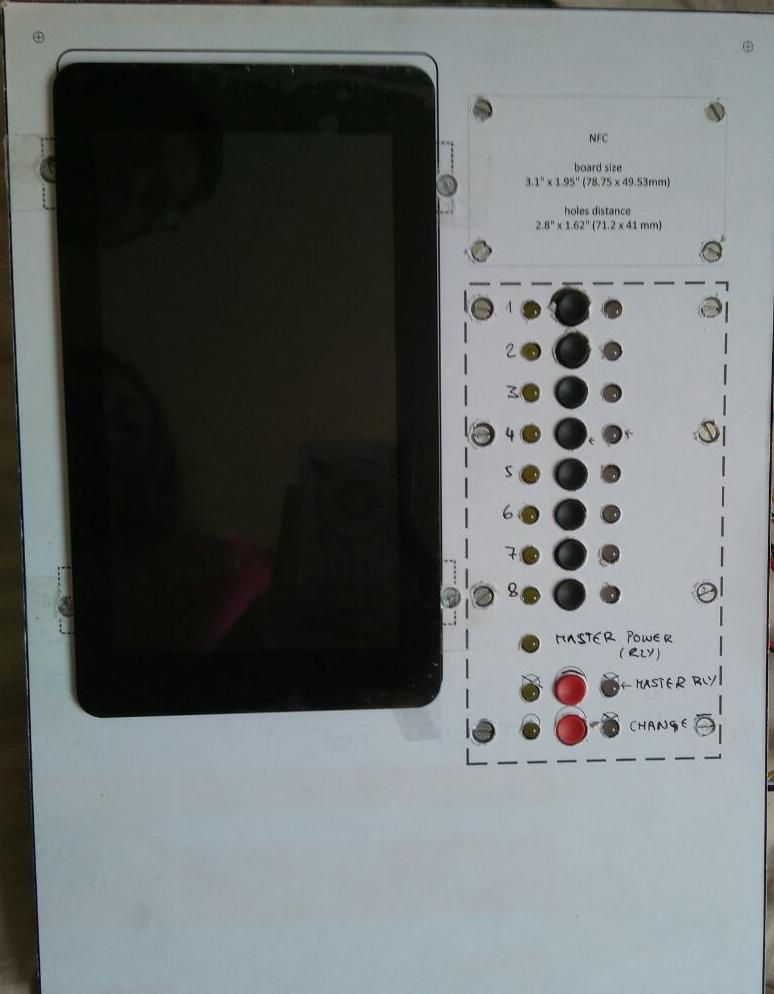
\includegraphics[width=0.8\textwidth]{images/demonstrator_front}
\caption{Interior de la unitat de test}
\label{fig:demonstrator_diagram}
\end{figure}

\begin{figure}
\center
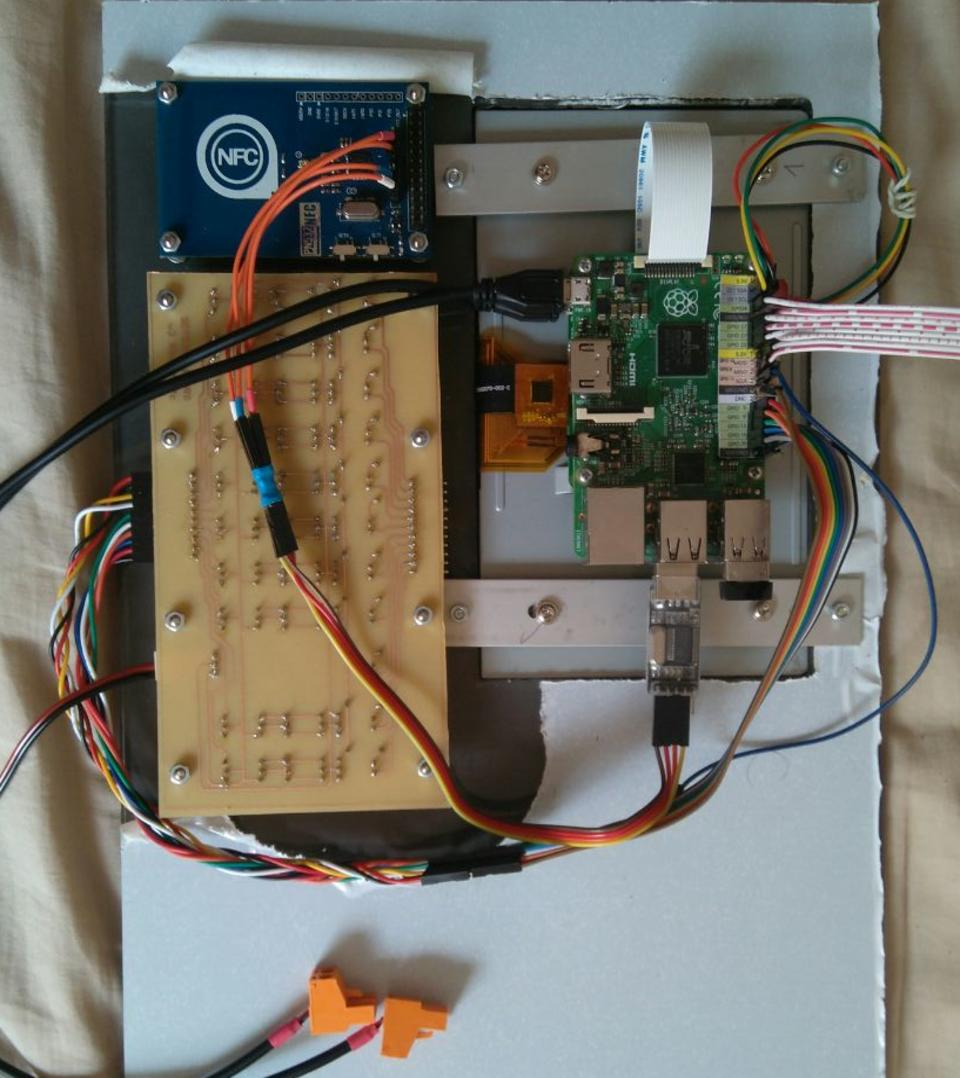
\includegraphics[width=0.8\textwidth]{images/demonstrator_back}
\caption{Interior de la unitat de test}
\label{fig:demonstrator_diagram}
\end{figure}

\begin{figure}
\center
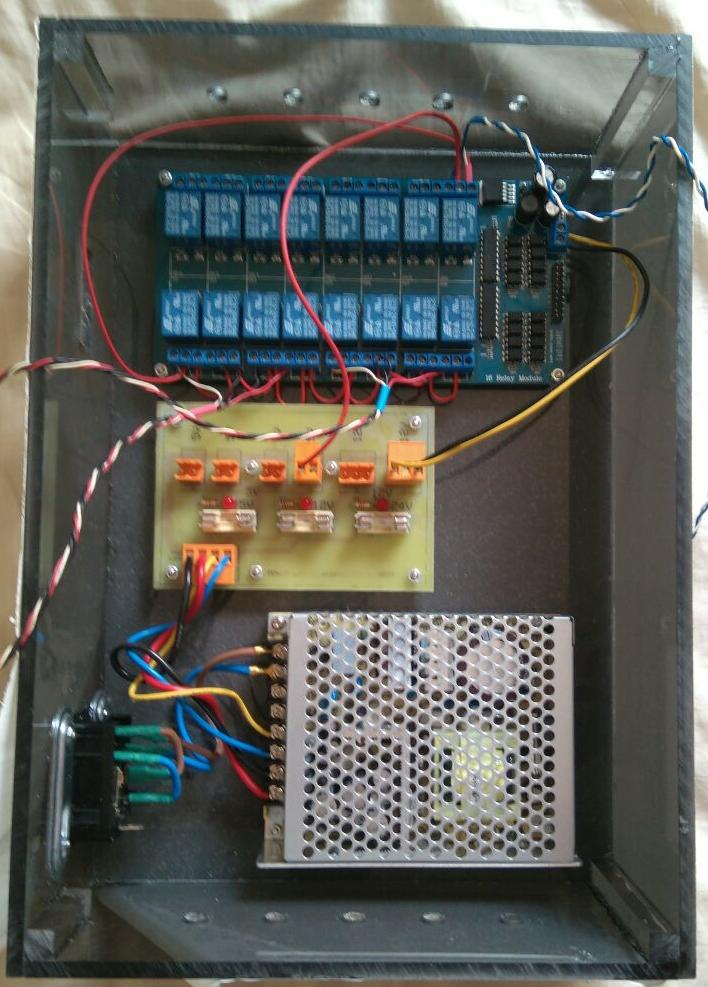
\includegraphics[width=0.8\textwidth]{images/demonstrator_bottom}
\caption{Interior de la unitat de test}
\label{fig:demonstrator_diagram}
\end{figure}
